\documentclass[11pt]{article}
\usepackage[margin=1in]{geometry}
\usepackage[numbers]{natbib}
\usepackage{graphicx}
\usepackage{amsmath}
\usepackage{amssymb}
\usepackage[parfill]{parskip} % new line between paragraphs, no indentation
\usepackage[colorlinks,pdfstartview=FitH,citecolor=blue, linkcolor=blue]{hyperref}
\usepackage{xcolor}
\usepackage{xeCJK} % Enabling Chinese characters
\usepackage{mdwlist} % Tight lists
\usepackage{enumerate} % Enabling options for list environments
\usepackage{float}


% Header
\usepackage{fancyhdr}
\pagestyle{fancy}
\fancyhf{}%Clear all heads and foots
\setlength{\headheight}{40pt} %Eliminate the warning of "headheight is too samll"
\rhead{Written Exam Answers\\Jianzhao Bi\\\today}
\cfoot{\thepage}

% Set font size for "section"
\usepackage{sectsty}
\sectionfont{\fontsize{11}{11}\selectfont}

% Define a new command for text subscript
\newcommand{\tsub}{\textsubscript}

\begin{document}

\section*{To Dr. Avani Wildani}
\setcounter{section}{0}

\section{In a single-sentence, how would you define your research question?}

\section{Missing satellite aerosol optical depth (AOD) data in Aim 1}
\begin{enumerate*}[{[a)]}]
    \item For the AOD over land surfaces, the major causes of missing data include (1) cloud cover, (2) snow/ice cover, (3) inland water bodies, and (4) no measurement (\textit{i.e.,} data points outside the satellite scanning range). These sources led to different proportions of missing data. Take New York State in 2015 as an example, the cloud-cover, snow-cover, no measurement, and inland water led to $\sim$75\%, $\sim$6\% (it increased to $\sim$20\% in the snow season), $\sim$10\%, and $< 1\%$ of missing AOD data, respectively. 
    
    The AOD observation could not be conducted in desert and semidesert regions by the original aerosol retrieval algorithm -- Dark Target (DT) \citep{kaufman1997modis, levy2007second}, because it was difficult to separate the aerosol signal from the top-of-atmosphere (TOA) reflectances at red and near-infrared wavelengths \citep{hsu2013enhanced}. Currently, a new algorithm -- Deep Blue (DB) \citep{hsu2004aerosol} utilizes blue wavelength where the surface reflectnace over land is much lower than for longer wavelength channels (\textit{i.e.,} red and near-infrared wavelengths). DB has successfully produced aerosol products over desert and semidesert areas and expanded the AOD availability to all cloud-free and snow/water-free land surfaces \citep{hsu2013enhanced}. 
    
    Major strategies dealing with the issue of missing AOD data can be classified as four categories. The first strategy is to adjust and improve current aerosol retrieval algorithms to increase available AOD estimations \citep{van2011satellite}. The second one is to utilize the spatiotemporal autocorrelation of AOD/PM\tsub{2.5} to interpolate the missing data by geostatistical interpolation approaches (\textit{e.g.,} universal kriging) \citep{kloog2011assessing, kloog2012incorporating}. The third one is using simulated AOD by chemical transport models in the regions without AOD measurements \citep{hu2017estimating}. The fourth one is to regress the missing AOD by statistical/machine learning models with AOD-related physical and land-use parameters (\textit{e.g.,} cloud fraction, meteorological parameters, elevation, \textit{etc.}) \citep{xiao2017full}.
    
    \item In my opinion, the biggest concern comes from the non-random nature of the missingness. It has been found that cloud and snow can lead to the change of AOD levels because of the shifted AOD physical characteristics under different meteorological conditions \citep{alam2014variability, kang2015correlation, emili2011high}. Thus, it may induce potential biases when missing AOD data are estimated only from existing AOD observations or under an incomplete consideration of the associations between cloud/snow and AOD. Considering the 90\% of missingness, this large proportion of potentially biased estimations might then affect the precision of PM\tsub{2.5} prediction in terms of its values and spatiotemporal patterns. For the health analyses, the measurement error of PM\tsub{2.5} can then lead to bias toward the null in estimated associations between PM\tsub{2.5} and its health outcomes \citep{sarnat2015fine}, that is, the underestimation of the adverse health effect of PM\tsub{2.5}.
    
    \item In this study, we are trying to reduce the systematic bias caused by the non-random missingness by incorporating AOD-related cloud/snow parameters in an appropriate statistical or machine learning model. For one thing, according to the validation of gap-filled AOD by the preciser ground-based AOD observations (\textit{i.e.,} AERONET data), utilizing the parameters relating to the cloud-/snow-AOD interactions (\textit{e.g.,} cloud/snow fractions) has been proven to be an effective way to estimate the systematic change of AOD levels and increase the precision of AOD estimation \citep{xiao2017full}. For another, an appropriate regression model is also key to an accurate gap-filling since the relationships between AOD and meteorological parameters are complex. The preliminary analysis of this study has shown that machine learning models (\textit{e.g.,} Random Forests and Neural Networks) performed much better than the multiple imputation model \citep{xiao2017full} which is a latest statistical model used in AOD gap-filling. This comparison indicates the advantage and potential of machine learning models dealing with complex interactions which can hardly be described by current statistical models. Admittedly, our current consideration about possible parameters explaining the cloud-/snow-AOD interactions is still limited and incomplete, and thus the bias will still exist in the AOD estimations. We will further examine more cloud/snow parameters and try to more precisely recover the relationships between cloud/snow and AOD.
\end{enumerate*}

\section{Low-cost sensor observations for \texorpdfstring{PM\tsub{2.5}}{PM2.5} predictions in Aim 2}
\begin{enumerate*}[{[a)]}]
    \item Yes. Based on some previous studies \citep{hu2017estimating, di2016assessing} and the preliminary results of this study, the convolutional layer of PM\tsub{2.5} measurements (applying a convolution kernel, here is an inverse distance weighting (IDW) kernel, on the input layer), as an additional predictor variable to account for spatial autocorrelation of PM\tsub{2.5}, has a larger contribution to the PM\tsub{2.5} predictions than satellite AOD data in the prediction models, and can significantly improve the model performance. Specifically, both \citet{hu2017estimating} and the preliminary analysis of this study showed that the PM\tsub{2.5} convolutional layers had the highest variable importance values in the PM\tsub{2.5} models based on the random forest algorithm. Similarly, in Equation 4 of the proposal, we are planning to produce a convolutional layer for low-cost sensor measurements which have a larger density than the regulatory stations, so it is expected to provide more detailed spatial patterns of PM\tsub{2.5} and have a significant contribution to the model performance. 
    
    \item Even though the PM\tsub{2.5} convolutional layer has greater influence and importance than satellite AOD in terms of the model performance, it cannot be said that satellite AOD is less important in the process of PM\tsub{2.5} estimation. The indicator of the model performance -- cross-validation -- can only be conducted in the areas with regulatory PM\tsub{2.5} stations, and these stations are currently unevenly distributed and only accumulated in the populated areas. Therefore, the model performance is unknown in the areas without regulatory stations, such as some rural areas and wild areas. As a result, it cannot be directly extrapolated that the PM\tsub{2.5} convolution is more important than the satellite data in these regions. In fact, since the satellite scans the land surfaces in the same way, unlike the PM\tsub{2.5} convolutional layer, it can provide a more stable data quality in both urban and rural areas. 
    
    Further, in order to assess the contribution of satellite AOD to the PM\tsub{2.5} predictions, we built a no-AOD prediction model in the preliminary analysis of this study. Figure \ref{fig:noaod} shows the spatial differences between full-model and no-AOD PM\tsub{2.5} in the snow season of 2015 (first 15 weeks). Compared to the no-AOD PM2.5, the full-model PM2.5 had changes in the spatial pattern with intensified on-road emissions. Hence, the pollution information provided by the satellite AOD can influence the PM\tsub{2.5} predictions in a discernible way. 
    
    \item If I had funds to invest in future data collection, I recommend first applying for the quality improvement of low-cost sensors, and then applying for the denser deployment of low-cost sensors, and finally applying for the development of new satellite sensors. In my opinion, this route can provide the quickest and most direct improvement for the PM\tsub{2.5} exposure assessment. Because of the smaller size and inexpensive deployment cost, the low-cost continuous monitoring instruments can potentially fill in gaps in the regulatory monitoring network to enhance the understanding of pollution hotspots \citep{gao2015distributed}. However, their large measurement errors hinder a wider application of them to assess compliance with air pollution standards \citep{hall2014integrating}. Once the low-cost sensors have reliable measurement qualities, it will be much easier to densely employ them to cover all population than the regulatory stations, and it might become the new ``regulatory'' measurements with high spatiotemporal coverage. Satellite sensors cannot provide direct obsevations of PM\tsub{2.5} so far, which limits their capability in PM\tsub{2.5} exposure assessment. However, satellite remote sensing can provide global-scale observation and are important to pollution event detection, transport and model prediction, and emission estimation \citep{hoff2009remote}, which are the unique advantages over the ground measurements. Consequently, satellite data are still valuable complements to the ground measurements, and with its evolving functions, it will play more important roles in the fields of environment and public health. 
\end{enumerate*}

\section{In your words, describe the specific parameter selection strategy for Equation 2}

\section*{To Dr. Stefanie Sarnat}
\setcounter{section}{0}

\section{How generalizable do you anticipate the \texorpdfstring{PM\tsub{2.5}}{PM2.5} models in Aims 1 and 2 to be?}
\begin{enumerate*}[{[a)]}]
    \item For the AOD gap-filling model (Equation 1), PM\tsub{2.5} prediction model (Equations 2), and PM\tsub{2.5} interpolation model (Equation 3), the generalizability mainly depends on the qualities of input data (\textit{i.e.,} satellite observations, regulatory measurements, meteorological data, and land-use data). In the United States, these datasets are well generated, validated, organized, and maintained, so they have good and stable data qualities. As a result, it is expected that these models are generalizable in the US. In fact, several studies \citep{kloog2011assessing, kloog2012incorporating, hu2017estimating, di2016assessing} have utilized similar models and datasets at regional and national scales in the US, generating high-resolution PM\tsub{2.5} predictions with good model performance. Further, the preliminary analysis of this study also applied these models in Imperial County, California, obtaining PM\tsub{2.5} predictions with similar performance as which in New York State. 
    
    For the PM\tsub{2.5} prediction model with low-cost sensor measurements (Equation 4), apart from the qualities of above-mentioned datasets, the availability of low-cost sensors is also key to the generalizability of the model. Figure \ref{fig:pa} shows the current distribution of PurpleAir low-cost monitors in the United States. According to the figure, the densest PurpleAir networks are on the west coast, especially in California, and in some eastern states, such as New York State, Pennsylvania, Maryland, North Carolina, \textit{etc.} For a regional-scale study, Equation 4 is expected to be generalizable to these states with dense PurpleAir networks. However, similar studies can only be conducted at local scales (such as county-level or city-level) in which there are limited low-cost sensors. 
    
    For the low-cost sensor calibration models (Equations 5 and 6), the generalizability should be further examined since no similar study has been conducted using these models for a nationwide, or even a statewide, low-cost sensor network. \citet{carvlin2017development} has calibrated Dylos PM sensors (Dylos Corporation, Riverside, CA) by regulatory measurements in Imperial County, California, showing that the measurement quality of the sensors is associated with meteorological conditions such as temperature and relative humidity. Studies \citep{broday2017wireless, castell2017can} also showed that the quality of laser-based PM\tsub{2.5} sensors is associated with particle size and PM composition. Therefore, our calibration models should be carefully tested, and adjusted if necessary, before generalize to other areas. 
    
    \item The limitation of generalizing Equations 1 -- 4 elsewhere mainly comes from the qualities of input data. In the areas with reliable input data, the PM\tsub{2.5} prediction is expected to be effectively conducted. For example, \citet{xiao2017full} used similar input datasets to estimate missing satellite AOD and PM\tsub{2.5} concentrations in Yangtze River Delta (YRD) of China in 2013 and 2014, which had good model performance with cross-validation R$^2$s of $\sim$0.8. In contrast, the preliminary analysis of this study used the same models in Lima, Peru to estimate PM\tsub{2.5} concentrations, but obtaining significantly worse model performance because of the lack of necessary data and limited data qualities and quantities. In order to maximize the prediction ability in this situation, the datasets should be carefully selected and the models should also be properly adjusted.
    
    The limitation of generalizing Equations 5 -- 6 mainly comes from the characteristics of specific low-cost sensors. For example, PM composition, relative humidity, and temperature may affect the precision of a sensor \citep{carvlin2017development, broday2017wireless, castell2017can}. The non-linear response to the PM\tsub{2.5} concentrations \citep{kelly2017ambient} and the quality degredation \citep{broday2017wireless} may also lead to the measurement errors. Thus, before applying to other regions, the calibration models should be examined, and then be adjusted according to the examination, such as adding appropriate covariates. 
\end{enumerate*}

\section{What factors might you be concerned about before using PurpleAir data?}
The most important factor having to be concerned about before using the data of the PurpleAir monitoring network is the quality of the PM\tsub{2.5} measurements. The methods of PM\tsub{2.5} measurement used in regulatory monitors are Federal Reference Method (FRM) or Federal Equivalent Method (FEM). This indicates that they have been developed to a clearly defined standard for PM\tsub{2.5} and have completed a rigorous testing and analysis protocol before they can be used to monitor compliance for the appropriate primary and/or secondary National Ambient Air Quality Standards (NAAQS) \citep{hall2014integrating}. On the contrary, no standard or protocol has been established for the newly emerged low-cost sensors, so their qualities cannot be guaranteed to assess compliance for NAAQS. For example, The maximum consistency errors of PurpleAir sensors (PA-II: Dual Laser Air Sensors) are $\pm$10\% in the range of 100 -- 500 $\mu g/m^3$ and $\pm$10 $\mu g/m^3$ in the range of 0 --100 $\mu g/m^3$. In this study, we plan to use two strategies to minimize the adverse effect of the low quality of PurpleAir sensors and to incorporate their measurements in the PM\tsub{2.5} prediction models:
\begin{enumerate*}[{[1)]}]
    \item \textbf{Using PurpleAir measurements as a predictor variable (an independent variable)}: In the benchmark approach of Aim 2, we will use the interpolated PurpleAir PM\tsub{2.5} measurements (by Equation 3) as a predictor variable in the PM\tsub{2.5} prediction model (Equation 4). This approach will not only utilize the spatial details of the measurements but also reduce the adverse effects of the measurement errors on the regression stage of the model. However, this approach will not increase the sample size of the dependent variable, so the model performance will still be limited if there are not enough regulatory PM\tsub{2.5} observations in the study domain. 
    \item \textbf{Calibrating the measurements and utilizing them as the dependent variable}: In order to increase the sample size of the dependent variable and fully utilizing the spatial details of the PurpleAir measurements, we plan to calibrate these data by the regulatory observations. The difficulties include the determination of an appropriate ``collocated'' distance between a PurpleAir sensor and the regulatory stations and the reliable extrapolation of the calibration coefficients. For the former problem, we will examine a series of distances and choose the most suitable one by cross-validation of the calibration model. For another problem, apart from the proposed kriging with external drift (KED) model, we will also test other interpolation methods (such as variational interpolation \citep{turk1999shape}) to obtain reasonable spatial representations of the calibration coefficients. 
\end{enumerate*}


% ----------- Figures ----------- %
\newpage
\begin{figure}[H]
    \centering
    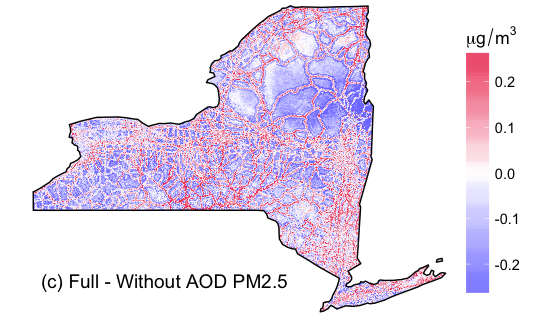
\includegraphics[width=0.7\textwidth]{img/no_aod.png}
    \caption{Spatial differences between full-model and no-AOD PM\tsub{2.5} in the snow season of 2015 (full-model minus no-AOD PM\tsub{2.5})}
    \label{fig:noaod}
\end{figure}

\begin{figure}[H]
    \centering
    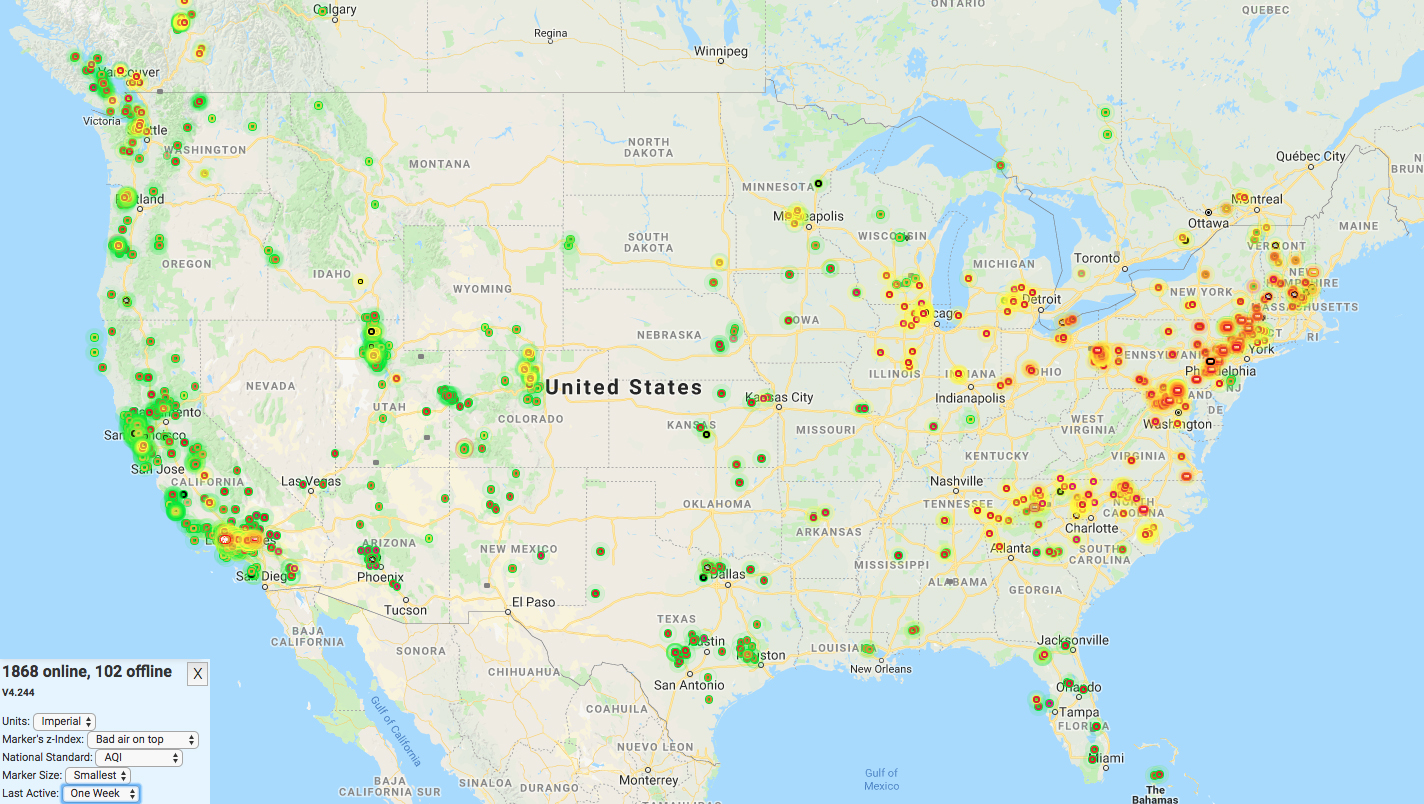
\includegraphics[width=0.9\textwidth]{img/purpleair.jpg}
    \caption{The distribution of PurpleAir low-cost sensors in the United States (Jun 19th, 2018)}
    \label{fig:pa}
\end{figure}

% ----------- References ----------- %
\newpage
\bibliographystyle{unsrtnat}
\bibliography{references}

\end{document}
